\chapter{Badania wstępne}
\label{cha:Badania wstępne}

Analiza rozpatrywanego problemu detekcji pozwoliła zawęzić przestrzeń rozważanych rozwiązań do wybranych typów warstw, architektur czy metod detekcji. 
Ponadto, na tej podstawie możliwe jest zaproponowanie własnego rozwiązania.
W niniejszym rozdziale zostaną przedstawione propozycje architektur sieci, proces ich uczenia, a także kwantyzacji. 

\section{Architektura wstępna}

Wspomniane w rozdziale \ref{subsec:sep_conv} konwolucje separowalne pozwalają zredukować liczbę parametrów sieci, a także wymaganą moc obliczeniową.
% Liczba parametrów sieci \emph{Ultra\_net} wynosi ponad 200 tys..
Przykładowo sieć \emph{SkyNet} ( wersji bez połączenia typu \emph{bypass}) wykorzystująca konwolucje separowalne posiada ponad $300$ tys. parametrów. 
Analogiczna architektura wykorzystująca pełną konwolucję posiada ponad $2.6$ miliona parametrów.
% (architektur tych jednak nie można w pełni ze sobą utożsamiać jako równoważnych). 
Tak znaczna redukcja (również złożoności obliczeniowej) skłania do zastosowania konwolucji separowalnych w przypadku akceleracji sprzętowej. 
% Jednakże liczba parametrów sieci \emph{SkyNet} dla wydajnej sprzętowej implementacji, wydaje się być wciąż nadmiarowa.
% Uzyskanie wydanej implementacji sprzętowej jest możliwe m.in. poprzez redukcję liczby parametrów.
Postanowiono również sprawdzić czy możliwa jest dalsza redukcja liczby parametrów pozwalająca na uzyskanie satysfakcjonującego wyniku detekcji.  
W tym celu rozważono architekturę sieci o 9 warstwach konwolucji separowalnej (z bias) z funkcją aktywacji $ReLU$ oraz  4 warstwami \emph{Max Pooling} umieszczonymi po wybranych konwolucjach separowalnych.
Ostatnia warstwa stanowi warstwę bazującą na warstwach \emph{YOLOv1} oraz \emph{YOLOv2} (rozdział \ref{ch:yolo}). 
Na rysunku \ref{fig:arch_v1} przedstawiono graficzną reprezentację architektury. 
Jako wejście sieci pozostawiono oryginalne wymiary obrazów dostępnych w zbiorze treningowym.

\begin{figure}
    \centering
    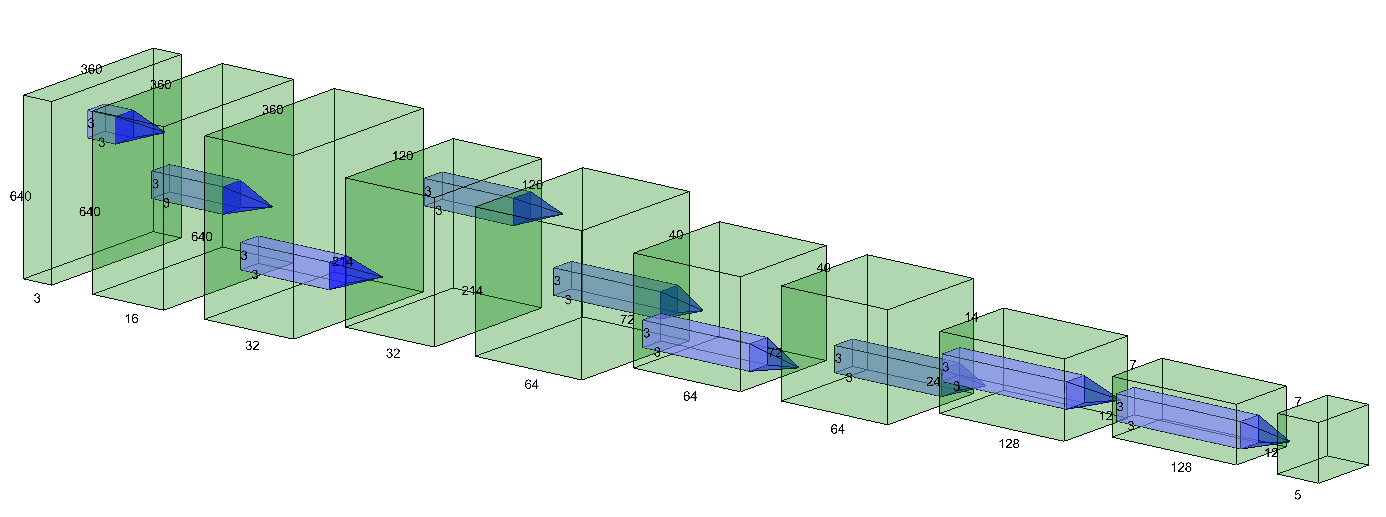
\includegraphics[width=\linewidth]{images/arch_v1.png}
    \caption{Wstępna architektura sieci dla zadania detekcji, wykorzystująca konwolucje separowalne oraz warstwę podobną do \emph{YOLOv1}. Architektura posiada niespełna 43 tys. parametrów.}
    \label{fig:arch_v1}
\end{figure}

Ze względu, iż rozpatrywany problem to detekcja bez klasyfikacji (przy czym wykrywane powinny być tylko obiekty należące do jednej z 12 klas), pominięto w funkcji błędu \eqref{eq:lossv1} część związaną z klasyfikacją. 
Obliczenie błędów poszczególnych neuronów jest realizowane poprzez porównanie z maską referencyjną wyjść $y_{ref}$ (o wymiarach $(5,d_h,d_w)$) z odpowiadającymi wartościami dla kanałów. 
Równania \eqref{eq:y_ref_valv1}-\eqref{eq:rowv1} prezentują sposób wyznaczenia wartości referencyjnych dla elementów poszczególnych kanałów oraz wyznaczenie położenia obiektu w siatce.

Poprzez $x_c, y_c, w, h$ oznaczono parametry obiektu referencyjnego, $a_w$ oraz $a_h$  odpowiednio szerokość i wysokość \emph{anchor box}, $W = 640$ oraz $H = 360$ wymiary obrazu wejściowego, $d_w = 12$ oraz $d_h = 7$ wymiary siatki detekcji. 
Przyjęto  $a_w = 16$ oraz $a_h = 16$ jako wartość łączną wartości kroku sieci (ang. \emph{stride}) wynikającą z liczby warstw \emph{Max Pooling}.

\begin{equation}
y_{ref}_{0,i,j} = 
\begin{cases}
    1, & \text{if }  i = row \land j = col \\
    0,              & \text{otherwise}
\end{cases}
\label{eq:y_ref_valv1}
\end{equation}

\begin{equation}
y_{ref}_{1,i,j} = 
\begin{cases}
    x_c \frac{d_w}{W} - col - 0.5, & \text{if }  i = row \land j = col \\
    0,              & \text{otherwise}
\end{cases}
\label{eq:y_ref_xv1}
\end{equation}

\begin{equation}
y_{ref}_{2,i,j} = 
\begin{cases}
    y_c \frac{d_h}{H} - row - 0.5, & \text{if }  i = row \land j = col \\
    0,              & \text{otherwise}
\end{cases}
\label{eq:y_ref_yv1}
\end{equation}

\begin{equation}
y_{ref}_{3,i,j} = 
\begin{cases}
    log(\frac{w}{a_w}) & \text{if }  i = row \land j = col \\
    0,              & \text{otherwise}
\end{cases}
\label{eq:y_ref_wv1}
\end{equation}

\begin{equation}
y_{ref}_{4,i,j} = 
\begin{cases}
    log(\frac{h}{a_h}) & \text{if }  i = row \land j = col \\
    0,              & \text{otherwise}
\end{cases}
\label{eq:y_ref_hv1}
\end{equation}

\begin{equation}
col = \round{x_c \frac{d_w}{W} - 0.5}
\label{eq:colv1}
\end{equation}
\begin{equation}
row = \round{y_c \frac{d_h}{H} - 0.5}
\label{eq:rowv1}
\end{equation}


Pierwszy kanał $y_{ref}_{0,:,:}$ oznacza referencyjną wartość dla wykrycia obiektu.
Zrezygnowano tutaj z wyznaczania wartości na podstawie $IoU$ i przyjęto tylko jeden element maski za niezerowy. 
Kolejnym kanałom dla elementu na pozycji $(row, col)$ przypisano odpowiednio przetransformowane parametry obiektu referencyjnego. Kanały $y_{ref}_{1:2,:,:}$ stanowią odchylenie środka obiektu od środka komórki (elementu $(row, col)$) siatki znormalizowane do wymiaru komórki siatki.
Kolejne dwa kanały $y_{ref}_{3:4,:,:}$ przedstawiają wykładnik przeskalowania eksponencjalnego wymiarów obiektu do wymiarów \emph{anchor box}.

Błąd wykrycia obiektu został zdefiniowany jako entropia binarna $BCE$ (ang. \emph{Binary Cross Entropy}). 
Błąd przesunięcia od centrum siatki detekcji oraz estymacja wymiarów został zdefiniowany jako średni błąd bezwzględny $MAE$ (ang. \emph{Mean Absolute Error}).
Funkcję błędu (reprezentowaną przez równanie \eqref{eq:lossv1}) dla całej sieci stanowi ważona suma błędów składowych ze współczynnikami $\lambda_obj, \lambda_xy oraz \lambda_wh$ dobieranymi w sposób eksperymentalny. 
Poprzez $y_{pred}$ oznaczono odpowiedź sieci. 

\begin{equation}
\begin{aligned}
loss =& \lambda_{obj} BCE(\sigma(y_{pred}_{0,:,:}), y_{ref}_{0,:,:}) \\
&+ \lambda_{xy}MAE(y_{pred}_{1:2,:,:}, y_{ref}_{1:2,:,:})\\
&+ \lambda_{wh}MAE(y_{pred}_{3:4,:,:},y_{ref}_{3:4,:,:}) 
\end{aligned}
\label{eq:lossv1}
\end{equation}


Przed rozpoczęciem procesu uczenia dokonano podziału dostępnego zbioru uczącego na trzy zbiory: uczący, walidacyjny oraz testowy w stosunku 81:9:10. 
Rozdzielenie danych odbywało się losowo wewnątrz każdej sekwencji.
Uzyskane zbiory były stosowane dla wszystkich dalszych wariantów architektur i funkcji błędu.

Rozpoczynając trening sieci ustalono wszystkie parametry funkcji błędu \eqref{eq:lossv1} na wartość $1$.
Dla zbioru uczącego przeprowadzano augmentację danych z wykorzystaniem filtracji uśredniającej (konwolucja z maską o wymiarze $SxS$ o wartościach $\frac{1}{S*S}$), zakłóceń addytywnych ( dodanie białego szumu z zakresu $[-\sigma;\sigma]$ z ograniczeniem wartości do przedziału $[0.0;1.0]$), przeskalowania (powiększenie lub pomniejszenie obrazu) czy też rotacji (obrót obrazu o kąt z zakresu $[-45\deg;45\deg]$).
Do minimalizacji błędu użyto algorytmu \emph{Adadelta}.
Dla pozostałych architektur również przeprowadzano augmentację danych i używano tego samego algorytmu optymalizacji.

Proces uczenia przerwano, gdy nie zauważono zmian wartości błędu oraz metryki \emph{IoU} dla zbioru uczącego oraz walidacyjnego.
Finalnie architektura osiągnęła wartość współczynnika $IoU = 0.47$ dla zbioru walidacyjnnego.
Uzyskany wynik był niesatysfakcjonujący, zdecydowano się na odrzucenie rozpatrywanej wersji architektury w dalszych rozważaniach.
W trakcie wizualizacji zauważono, iż sieć poprawnie wskazuje element siatki, lecz gorzej radzi sobie regresją parametrów.
Przyczyną mogła być zbyt rzadka siatka detekcji.

\section{Architektura rozgałęziona}

Architektura \emph{SSD} wykorzystuje połączenia pochodzące z warstw pośrednich celem poprawienia rezultatów detekcji.  
Ze względu na niewielką wartość współczynnika $IoU$, wcześniej rozważaną architekturę zmodyfikowano o  dodatkowe wyjście z sieci pochodzące z warstwy pośredniej zakończonego warstwą \emph{YOLO} analogicznie jak w wersji nierozgałęzionej (wymiary \emph{anchor box} dla rozgałęzienia $a_w = 8$ oraz  $a_h = 8$). 
Na rysunku \ref{fig:arch_v2} przedstawiono graficzną reprezentację architektury. 
Po przeprowadzeniu procesu ucznia sieci, z wykorzystaniem techniki transferu wiedzy z architektury pierwotnej, uzyskano pogorszenie wartości $IoU$.
Z tego powodu odrzucono analizę również tej architektury.
Przyczyną niepowodzenia może być zbyt mała liczba parametrów dla rozpatrywanego problemu.
Ponadto w stosowanych funkcjach błędu dla części regresyjnej wymagano zerowych rezultatów (wartość referencyjną stanowiło 0 ) elementów siatki, do których nie przypisano obiektu (położenie różne od $(row,col)$).
Zwiększa to stabilność działania sieci, jednakże wymaga również większej liczby pozytywnych detekcji z parametrami różnymi od wymiaru \emph{anchor box} oraz położenia środka elementu siatki, co dla rozpatrywanego problemu detekcji pojedynczego obiektu nie jest możliwe. 

\begin{figure}
    \centering
    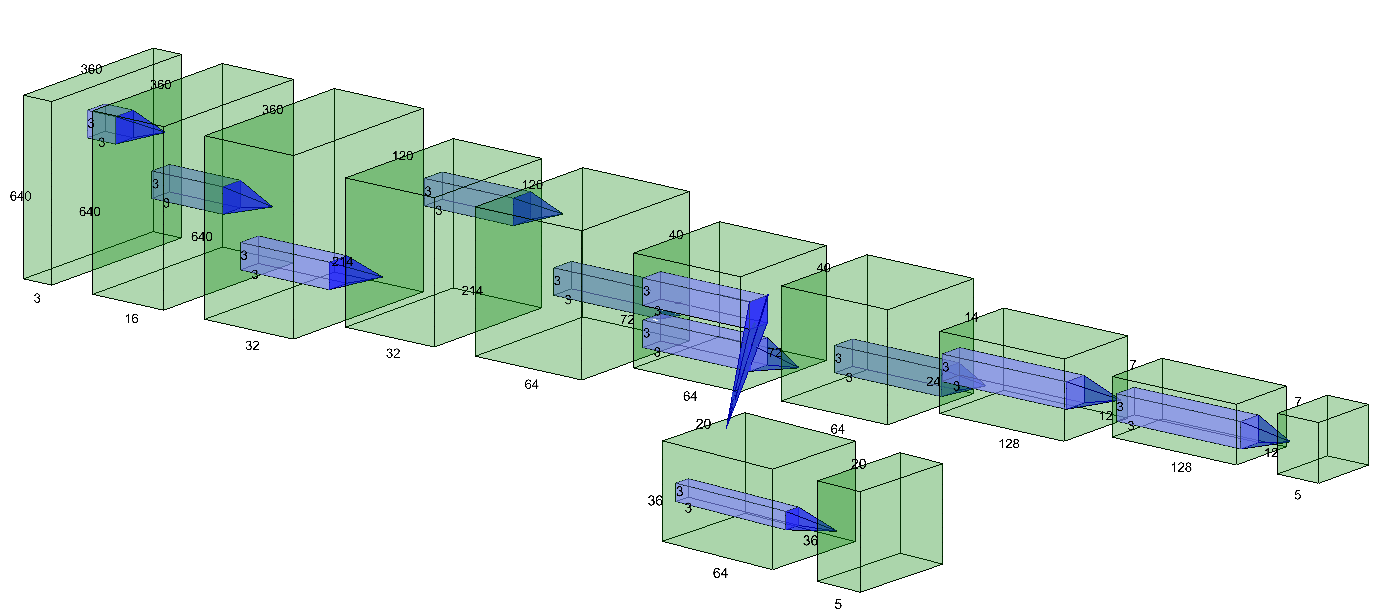
\includegraphics[width=\linewidth]{images/Architektura_branched.png}
    \caption{Architektura rozgałęziona wykorzystująca konwolucje separowalne.}
    \label{fig:arch_v2}
\end{figure}


\section{Architektura Resnet18}

\begin{figure}
    \centering
    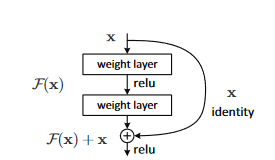
\includegraphics{images/residual.png}
    \caption{Blok rezydualny. Przekształcenie identycznościowe omijające wybrane bloki konwolucji. Źródlo: \cite{resnet18}}
    \label{fig:res_block}
\end{figure}

Rezultaty dotychczas badanych architektur były niesatysfakcjonujące.
Zdecydowano się zatem na zastosowanie rozwiązania o znacznie większej liczbie parametrów, a także wykorzystującego połączenia rezydualne (połączenia omijające wybrane następne warstwy przedstawione na rysunku \ref{fig:res_block} )- \emph{Resnet18}\cite{resnet18}, tym samym sprawdzając czy bardziej rozbudowany model uzyska żądane rezultaty. 
W tym celu wykorzystano dwa pierwsze bloki rezydualne sieci \emph{ResNet18} wraz z dodatkową warstwę konwolucyjną posiadającą 128 filtrów oraz warstwą \emph{YOLOv3}. 
Celem przyspieszenia procesu uczenia wagi bloków rezydualnych zostały zainicjalizowane wagami z sieci trenowanej na zbiorze \emph{ImageNet}\cite{imagenet} (dostęp za pośrednictwem biblioteki \emph{PyTorch}).
Wykorzystano tu trzy \emph{anchor box} o wymiarach (szerokość x wysokość): $22x33, 43x69, 89x133$ uzyskanych jako wynik algorytmu k-średnich. 
Uzyskana architektura podsiadała ponad 700 tys. parametrów.
Wymiary obrazów wejściowych zredukowano do 360 pikseli szerokości oraz 180 pikseli wysokości.
Funkcja błędu odpowiedzi sieci przyjmuje postać daną równaniem \eqref{eq:loss_yolo_resnet}.
Jako funkcję błędu regresji wybrano funkcję \emph{GIoU} \eqref{eq:giou}.
Błąd wykrycia obiektu jest realizowany przez funkcję entropii binarnej.
Dla obu współczynników wagowych przyjęto wartość $1$.
\begin{equation}
loss(v_{pred},v_{ref},A_{pred}, B_{ref}) = \lambda_{validity} BCE(v_{pred}, v_{ref}) + \lambda_{bbox} \sum_{a = 0}^{2} GIoU(A_{pred}(a), B_{ref})
\label{eq:loss_yolo_resnet}
\end{equation}
Poprzez $v_{pred}$ oznaczono 3 kanały wykrycia obiektu dla każdego \emph{anchor box}, 
$v_{ref}$ stanowi maskę referencyjną.
Wartość $1$ znajduje się na pozycji $(row,col)$ (wyznaczane z równań \eqref{eq:rowv1}-\eqref{eq:colv1}) dla każdego \emph{anchor box}.
Predykcja parametrów obiektu dla elementu siatki $(row,col)$ dla $a$-tego \emph{bounding box} została oznaczona $A_{pred}(a)$ oraz wyznaczona za pomocą równań \eqref{eq:xc_yolov2}-\eqref{eq:h_yolov2}.
Parametry obiektu referencyjnego oznaczono poprzez $B_{ref}$. 
Wyznaczany błąd jest obliczany względem grupy filtrów każdego z \emph{anchor box} na tej samej pozycji w siatce.


Dla modelu zmiennoprzecinkowego architektura osiągnęła wartość $IoU$ ponad $0.8$ dla zbioru walidacyjnego. Proces uczenia został przerwany podobnie jak poprzednio, gdy nie zauważano znaczących zmian błędu i metryki \emph{IoU}.

Zdecydowano się na kwantyzację modelu z wykorzystaniem zapisu stałoprzecinkowego z wartościami dobranymi eksperymentalnie. 
Obraz wejściowy (znormalizowany do przedziału $[0.0;1.0]$) został poddany kwantyzacji 8 bitowej bez znaku i bez części całkowitej. 
Wagi oraz wyjścia warstw pośrednich poddano kwantyzacji 8 bitowej ze znakiem i 2 bitami części całkowitej.
Ostanie dwie warstwy poddano kwantyzacji 8 bitowej ze znakiem i 3 bitami części całkowitej (możliwość uzyskania skali przekształcającej \emph{anchor box} do wymiarów obrazu).
W przypadku każdej kwantyzacji zastosowano również ograniczenie wartości wynikowej do limitów wynikających z zapisu w formacie stałoprzecinkowym. 
Tak dobrane parametry kwantyzacji mają również pełnić zadanie pewnego rodzaju regularyzacji.

Po zakończeniu treningu sieci z kwantyzacją osiągnięto wartość $IoU = 0.72$.
Uzyskana wartość pozwalałaby na osiągnięcie maksymalnej wartości oceny 
danej równaniem \eqref{eq:iou_score} (jeżeli uzyskano by podobny rezultat na zbiorze tajnym).

Rozważana architektura wydaje się być trudniejsza do sprzętowej implementacji ze względu na połączenia rezydualne oraz znaczne rozmiary. 
Jednakże analizując przeprowadzone procesy uczenia można zauważyć, iż dodanie warstw normalizujących oraz zastosowanie funkcji błędu bazującej na metryce \emph{IoU} pozwala na osiągnięcie większych wartości \emph{IoU}, przy mniejszej liczbie epok treningowych 
(dla poprzednich architektur liczba epok treningowych była znacząco większa, niż dla architektury rezydualnej). 


\section{LittleNet}
\label{ch:LN}

Podsumowując wnioski z rozważanych dotychczas architektur można stwierdzić, iż:
\begin{itemize}
    \item zastosowanie konwolucji separowalnych pozwala na znaczną redukcję liczby parametrów oraz złożoności obliczeniowej, 
    \item warstwy normalizacji pozwalają zmniejszyć liczbę epok treningowych,
    \item funkcja błędu bazująca na matryce \emph{IoU} pozwala osiągnąć lepsze wyniki.
\end{itemize}

Dodatkowo można zauważyć, iż konwolucja separowalna dla pierwszej warstwy posiada jedynie trzy filtry \emph{DW}.
Zatem następna warstwa \emph{PW} dokonuje podziału w przestrzeni zaledwie trójwymiarowej. 
Może to skutkować utratą znaczącej części informacji już na początkowym etapie przetwarzania, a także redundancją filtrów \emph{PW} (w przypadku większej ich liczby).
Zastosowanie pełnej konwolucji w pierwszej warstwie mogłoby polepszyć jakość detekcji.
Jednakże kownolucje pełne są bardziej złożone w implementacji sprzętowej. 
Z tego względu zdecydowano się na zastosowanie wielokrotnej filtracji \emph{DW}.
Wówczas każdy kanał wejściowy jest filtrowany nie jednym, a $m$ niezależnymi filtrami.
Pozwala to na zwiększenie liczby cech kontekstowych bezpośrednio ekstrahowanych z obrazu (czy też z każdego kanału) wraz z zachowaniem możliwości stosunkowo łatwej implementacji sprzętowej.

Proponowaną architekturę przedstawiono na rysunku \ref{fig:LN_arch}. 
Projekt architektury powstał wychodzą z architektury \emph{SkyNet} \cite{skynet}, 
poprzez dodanie dodatkowej warstwy konwolucji oraz eksperymentalnie dobranych wymiarów warstw, mając na uwadze redukcję liczby parametrów architektury wyjściowej. 
Sieć zawiera 7 bloków z konwolucją \emph{DW} oraz 7 z konwolucją \emph{PW}. 
Po każdej konwolucji występuje warstwa normalizacyjna oraz funkcja aktywacji $ReLU$. 
Pierwszy blok zawiera warstwę \emph{DW} z pięciokrotną filtracją kanałów, kolejne bloki zawierają już tylko dwukrotną filtrację kanałów.
Po pierwszych 4 warstwach \emph{PW} występuje warstwa \emph{Max Pooling}. 
Ostatnią warstwę stanowi konwolucja \emph{PW} stanowiąca warstwę \emph{YOLOv3}. 
Wymiary \emph{anchor box} pozostały takie same jak dla architektury wykorzystującej bloki rezydualne, lecz przeskalowane do wymiarów wejścia sieci. 
Proponowana architektura posiada niespełna 134 tys. parametrów, co stanowi znaczą redukcję liczby parametrów w stosunku do \emph{SkyNet} (powyżej 300 tys.) oraz \emph{Ultra\_net} (ponad 200 tys.). 
Architekturze nadano % roboczą
nazwę \emph{LittleNet} (\emph{LN}).
\begin{figure}
    \centering
    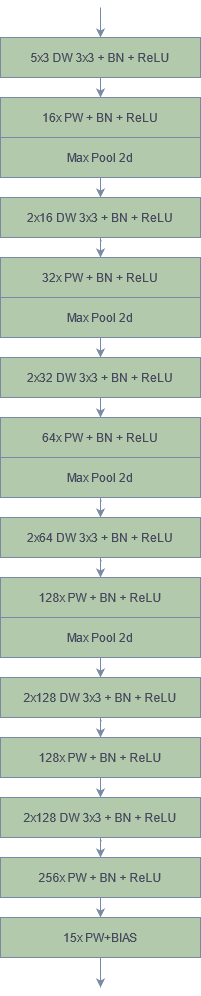
\includegraphics[width=4cm]{images/LNv1}
    \caption{Proponowana architektura sieci \emph{LittleNet}.}
    \label{fig:LN_arch}
\end{figure}

Rozmiar wejścia sieci ustalono na 360 pikseli szerokości oraz 180 pikseli wysokości.
Funkcja błędu odpowiedzi sieci \eqref{eq:loss_yolo_resnet} rozszerzono o regularyzację normą $L_1$ (średnia wartość bezwzględna) parametrów sieci $p$ oraz uogólnienie błędu regresji funkcją $IoU_{based}$, uzyskując równanie \eqref{eq:loss_LN}.
\begin{equation}
\begin{aligned}
loss(v_{pred},v_{ref},A_{pred}, B_{ref}, p) 
=& \lambda_{validity} BCE(v_{pred}, v_{ref} \\
&+ \lambda_{bbox} \sum_{a = 0}^{2} IoU_{based}(A_{pred}(a), B_{ref}) \\
&+ \lambda_{reg} L_1(p)
\end{aligned}
\label{eq:loss_LN}
\end{equation}
Za funkcję błędu regresji $IoU_{based}$ przyjęto funkcję \emph{GCIoU}(ang. \emph{Generalized Complete IoU}) daną równaniem \eqref{eq:gciou}. 
Funkcja ta bazuje na \emph{GIoU}\cite{giou}, \emph{DIoU}\cite{dciou} oraz \emph{CIoU}\cite{dciou}. 
Połączenie powyższych funkcji pozwala na połączenie ich zalet funkcji wraz z eliminacją wad: 
\begin{itemize}
    \item $giou_{part}$ - bardziej bezpośredni wpływ na parametry oraz poprawne skalowanie (gdy \emph{IoU}$ = 0$) \eqref{eq:giou_part},
    \item $diou_{part}$ - centralizacji predykcji \eqref{eq:diou_part},
    \item $ciou_{part}$ - wzmocnione finalne skalowanie rozmiaru \eqref{eq:ciou_part}. 
\end{itemize}
\begin{equation}
\begin{aligned}
GCIoU(A,B) =& 1 - IoU(A,B) + giou_{part}(A,B)\\ 
&+ diou_{part}(A,B) + ciou_{part}(A,B)
\end{aligned}
\label{eq:gciou}
\end{equation}
Ustalono parametry wagowe na $\lambda_{validity} = 20$, $\lambda_{bbox} = 1$ oraz $\lambda_{reg} = 0.01$ (bazując na rozwiązaniu \cite{ultra_net}).
Krok uczący został początkowo ustalony jako $l_r(0)=1$. 
W trakcie procesu uczenia podlegał on modyfikacji zgodnie z równaniami \eqref{eq:lr_1} oraz \eqref{eq:lr_2}.
Poprzez $t$ oznaczono numer epoki uczącej, natomiast $loss(t)$ oznacza średnią wartość funkcji błędu na zbiorze uczącym po epoce $t$.
Tak przeprowadzana zmiana kroku uczącego pozwala na dokonywanie większych zmian wag, gdy możliwe było zmniejszenie błędu oraz mniejsze zmiany, gdy wartość błędu wzrosła.
\begin{equation}
l_r_(t+1) = 
\begin{cases}
    1.3*l_r(t), &\text{if } loss(t) < loss(t-1) \\
    0.5*l_r(t), &\text{if } loss(t) > loss(t-1) \\
    l_r(t), &\text{otherwise}
\end{cases}
\label{eq:lr_1}
\end{equation}
\begin{equation}
l_r(t+1) = max(10^{-5}, min(1, l_r(t+1)))
\label{eq:lr_2}
\end{equation}


Po zakończeniu procesu uczenia modelu zmiennoprzecinkowego osiągnięto wartość $IoU = 0.8$ dla zbioru walidacyjnego oraz $0.7$ dla zbioru uczącego. 
Powodem tak znacznej różnicy wartości metryki jest znaczny stopień augmentacji danych.

Następnie sieć poddano kwantyzacji. 
Dane wejściowe zostały poddane kwantyzacji 8 bitowej bez znaku i bez części całkowitej.
Warstwy pośrednie poddano kwantyzacji 8 bitowej ze znakiem i 2 bitami części całkowitej.
Ostatnią warstwę poddano kwantyzacji 8 bitowej ze znakiem i 3 bitami części całkowitej.

Uzyskano wartość $IoU = 0.76$ dla zbioru walidacyjnego oraz $0.67$ dla zbioru uczącego.
Na rysunkach \ref{fig:float_loss}-\ref{fig:quant_iou} przedstawiono przebiegi funkcji błędu oraz metryki \emph{IoU} dla modelu zmiennoprzecinkowego oraz kwantyzowanego.

\begin{figure}
     \centering
     \begin{subfigure}[b]{0.49\textwidth}
         \centering
         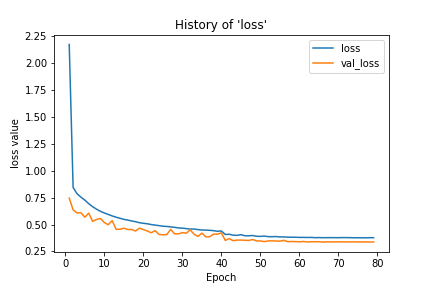
\includegraphics[width=\textwidth]{images/float32_hist_of_loss.png}
         \caption{}
         \label{fig:float_loss}
     \end{subfigure}
     \hfill
     \begin{subfigure}[b]{0.49\textwidth}
         \centering
         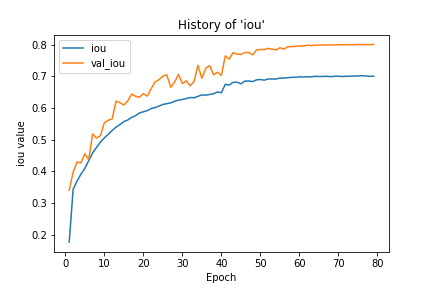
\includegraphics[width=\textwidth]{images/float32_hist_of_iou.png}
         \caption{}
         \label{fig:float_iou}
     \end{subfigure}
     \hfill
     \begin{subfigure}[b]{0.49\textwidth}
         \centering
         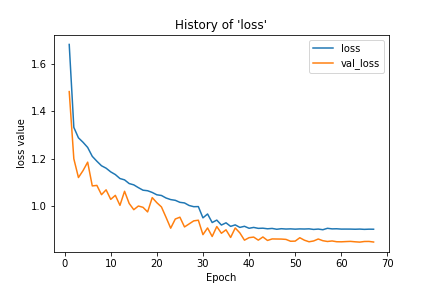
\includegraphics[width=\textwidth]{images/8_bit_quant_hist_of_loss.png}
         \caption{}
         \label{fig:quant_loss}
     \end{subfigure}
     \hfill
     \begin{subfigure}[b]{0.49\textwidth}
         \centering
         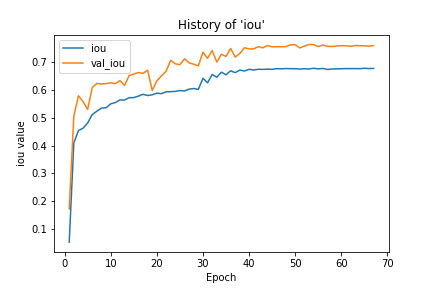
\includegraphics[width=\textwidth]{images/8_bit_quant_hist_of_iou.png}
         \caption{}
         \label{fig:quant_iou}
     \end{subfigure}
     \hfill
     
    \caption{Przebiegi wartości błędu oraz metryki \emph{IoU} (w zależności od epoki uczącej) dla modelu zmiennoprzecinkowego \ref{fig:float_loss} i \ref{fig:float_iou} oraz \ref{fig:quant_loss} i \ref{fig:quant_iou}.}
    \label{fig:two_step_train}
\end{figure}


W trakcie realizacji implementacji sprzętowej, ustalono, iż dla obecnego rozmiaru wejścia sieci nie jest możliwe buforowanie wyników warstw pośrednich w pamięci BRAM.
Z tego względu zdecydowano się na redukcję rozmiaru wejścia sieci do 200 pikseli szerokości oraz 100 pikseli wysokości. 
Rozpoczęto trening sieci z takimi samymi parametrami (wagi sieci zostały wylosowane).  
Uzyskano wartość $IoU = 0.78$ dla zbioru walidacyjnego oraz $0.69$ dla zbioru uczącego.

Eksperymentalnie stwierdzono również, iż parametry warstw normalizacyjnych po przekształceniu do formy afinicznej uzyskują w większości przypadków wartości przekraczające zadany zakres wartości wynikający z dotychczasowej kwantyzacji.
Względem poprzedniego modelu zmieniono liczbę bitów części całkowitej: 1 dla wyjść oraz 3 dla wag warstw pośrednich.
Od epoki $75$ rozpoczęto kwantyzację z wyłączeniem warstw normalizujących.
Następnie od epoki $109$ kwantyzacji poddano również warstwy normalizujące.
Dla modelu w pełni kwantyzowanego uzyskano wartość $IoU = 0.71$ dla zbioru walidacyjnego oraz $0.64$ dla zbioru uczącego. 
Na rysunkach \ref{fig:small_loss}-\ref{fig:small_iou} przedstawiono przebiegi funkcji błędu oraz metryki \emph{IoU} dla modelu o zmniejszonych rozmiarach wejścia. 

\begin{figure}
     \centering
     \begin{subfigure}[b]{0.49\textwidth}
         \centering
         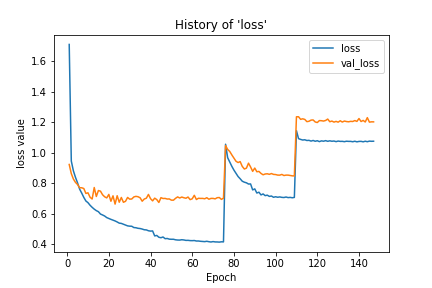
\includegraphics[width=\textwidth]{images/LN_smaller_hist_of_loss.png}
         \caption{}
         \label{fig:small_loss}
     \end{subfigure}
     \hfill
     \begin{subfigure}[b]{0.49\textwidth}
         \centering
         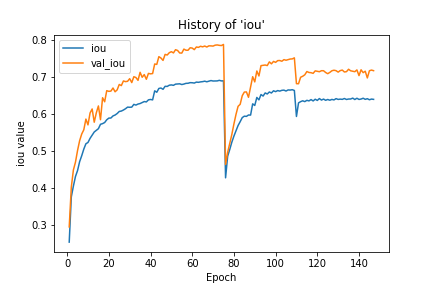
\includegraphics[width=\textwidth]{images/LN_smaller_hist_of_iou.png}
         \caption{}
         \label{fig:small_iou}
     \end{subfigure}
     
    \caption{Przebiegi wartości błędu \ref{fig:small_loss} oraz metryki \emph{IoU} \ref{fig:small_iou} (w zależności od epoki uczącej) dla modelu o rozmiarze wejścia 200x100 pikseli.
    Epoka 75 -- rozpoczęcie kwantyzacji bez warstw normalizacyjnych. Epoka 109 -- pełna kwantyzacja.}
    \label{fig:three_step_train}
\end{figure}


%  Podsumowanie
Poprzez analizę przeprowadzonych badań architektury stwierdzono, iż stosowanie konwolucji separowalnych posiada zaletę w postaci stosunkowo niewielkiej liczby parametrów, lecz również wadę wynikającą ze stosunkowo niewielkiego stopnia ekstrakcji cech z danych wejściowych (w szczególności w warstwach początkowych). 
Problem ten rozwiązano poprzez wielokrotną filtrację filtrami \emph{depthwise}.
Ponadto zastosowanie warstw normalizacyjnych pozwoliło na przyspieszenie procesu uczenia.
Wykorzystując wnioski z przeprowadzonych badań zaprojektowano architekturę \emph{LittleNet}.
Jako funkcję błędu regresji zaproponowano własne rozwiązanie (\emph{GCIoU}) bazującą na już istniejących.
Osiągnięto dokładność $IoU = 0.71$ wraz z możliwą stosunkowo prostą implementacją sprzętową.
Poza przedstawionymi przeprowadzono wiele innych eksperymentów, 
których rezultaty nie pozwalały osiągnąć większych wartości $IoU$.
Na tej podstawie oraz na podstawie dotychczasowych wyników konkursu ($IoU \leq 0.74$) stwierdzono, 
iż uzyskanie wartości wyższych jest stosunkowo trudne dla niewielkich architektur implementowanych sprzętowo.
Z tego względu zaakceptowano uzyskany rezultat jako zadawalający.